\capitulo{5}{Aspectos relevantes del proyecto} 
\label{capitulo5}

\newcommand{\kw}[1]{\texttt{#1}}
\newcommand{\code}[1]{\texttt{#1}}

El comienzo del proyecto parte del objetivo de conseguir una versión MVP (\emph{Minimal Viable Product}) que pudiese aportar una base sólida y fácil de ampliar. En este caso el MVP se enfocó en la creación de un micro compilador capaz de procesar expresiones aritméticas y lógicas, puesto que esta estructura es básica que está presente en todos los lenguajes de programación.

En fases posteriores del proyecto se trabaja tomando como base este MVP para añadir características adicionales al lenguaje, como las estructuras de control condicionales, bucles, funciones y eventos.

Es importante como paso previo a la creación de un lenguaje, la elección de un nombre para el mismo. Puesto que el objetivo inicial del proyecto implicaba experimentar con estructuras lógicas dependientes del tiempo y teniendo en cuenta la presencia de un tipo temporal en el lenguaje, se ha elegido el nombre «T» para el lenguaje y «Tcompiler» para el compilador, la sencillez de este nombre viene inspirada por el lenguaje C.

\subsection{Antes de compilar} 
El compilador antes de comenzar el proceso de compilación debe recibir en su ejecución datos que hagan referencia al archivo que se debe compilar, que archivo de salida se quiere generar y de que forma se debe realizar el proceso, permitiendo así al programador ajustar este proceso a sus necesidades.

Dentro del compilador se esperan algunos argumentos de llamada como:
\begin{itemize}
    \item \texttt{\textbf{<nombre de la entrada>}}: argumento obligatorio, indica el nombre del fichero \kw{.T} de entrada.
    \item \texttt{\textbf{-o <nombre archivo>}}: argumento obligatorio que especificar el fichero ejecutable de salida.
    \item \texttt{\textbf{-{}-debug}}: permite ver información de la salida de cada una de las fases del compilador. Este argumento también activa el efecto del argumento \code{-{}-visualizeAST};
    \item \texttt{\textbf{-{}-visualizeAST}}: genera un fichero \kw{AST.pfd} con una visualización del AST en el directorio donde se ha ejecutado el compilador.
    \item \texttt{\textbf{-{}-IR <nombre archivo>}}: genera un fichero \kw{.ll} con el LLVM IR generado por el compilador.
    \item \texttt{\textbf{-{}-basic}}: excluye la fase de optimización del proceso de compilación.
    \item \texttt{\textbf{-{}-help / -h}}: muestra la ayuda del compilador, indicando como debe ser utilizado y sus diferentes argumentos.
    \item \texttt{\textbf{-{}-version / -v}}: muestra la versión actual del compilador.
\end{itemize}

Para conocer los datos necesarios para ejecutar los comandos anteriores en el compilador se almacenan flags de compilado que permiten modificar el comportamiento de cada fase.

\subsection{Proceso de compilación}
Como el compilador se ha planificado de forma modular, a continuación se recorrerá el proceso de compilación completo, utilizando del contenido del MVP como ejemplo.

\subsubsection{Análisis léxico}
El analizador léxico lo generaremos mediante la herramienta ANTLR4, la cual nos permite definir los lexemas del lenguaje de forma independiente de la producciones gramaticales donde se van a utilizar. En este proyecto, el archivo que contiene esta información se encuentra en \texttt{src/grammar/Tlexer.g4}.

En este momento se definen las palabras clave asociadas a los tipos básicos del lenguaje:
\begin{minted}{ANTLR}
    TYPE_INT     : 'int'    ;
    TYPE_FLOAT   : 'float'  ;
    TYPE_CHAR    : 'char'   ;
    TYPE_STRING  : 'string' ;
    TYPE_BOOLEAN : 'bool'   ;
    TYPE_VOID    : 'void'   ;
    TYPE_PTR     : 'ptr'    ;
\end{minted}

Se definen los operadores aritméticos y lógicos:
\begin{minted}{ANTLR}
    PLUS  : '+' ;
    MINUS : '-' ;
    MUL   : '*' ;
    DIV   : '/' ;
    MOD   : '%' ;

    INC   : '++' ;
    DEC   : '--' ;

    EQ : '==' ;
    NE : '!=' ;
    LT : '<'  ;
    LE : '<=' ;
    GT : '>'  ;
    GE : '>=' ;
\end{minted}

\subsubsection{Análisis sintáctico}
Una vez obtenido el analizador léxico el siguiente paso es construir un analizador sintáctico capaz de reconocer producciones gramaticales, al igual que en la fase anterior, se realiza con ANTLR4 y se define el archivo \texttt{src/grammar/Tparser.g4}.

Los operadores y las operaciones se definen en el lenguaje ANTLR4 de la siguiente forma:
\begin{minted}{ANTLR}
expr
    : expr op=(MUL|DIV) expr        # arithmeticExpr
    | expr op=(PLUS|MINUS) expr     # arithmeticExpr
    | expr comparisonOperator expr  # logicalExpr
    | operand                       # operandExpr
    | LPAREN expr RPAREN            # parenExpr
    ;

comparisonOperator
    : EQ 
    | NE
    | LT 
    | LE 
    | GT
    | GE
    ;

operand
    : literal
    ;
\end{minted}
Cabe destacar el uso de etiquetas (como \code{\# parenExpr}) que facilitan posteriormente acceder a cada tipo de expresión gracias a la separación en contextos que realiza ANTLR4. En este ejemplo en concreto, la etiqueta \code{\# arithmeticExpr} sirve para separar la precedencia, permitiendo empaquetar en el mismo contexto ambas producciones, facilitando el análisis en fases posteriores.

\subsubsection{Generación del AST}
Para formar el AST se empleará un \eng{visitor pattern} (patrón de visita), objeto que recibe el nombre de \kw{ASTBuilder}, el cual se encarga de visitar cada contexto generado de forma automática por el parser de ANTLR, dando por resultado una estructura de nodos enlazados, el AST.

Adicionalmente, si la flag \code{-{}-visualizeAST} está activada, el compilador puede generar una representación visual del árbol tras su construcción, para conseguir esto se escriben cada nodo en el formato de la biblioteca `forest` de \LaTeX, permitiendo el análisis de la estructura del programa así como datos relacionados con los componentes, como los tipos u operadores.

\label{capitulo5:AST}
\imagen{AST_ejemplo_expr}{Ejemplo de visualización de la expresión 2 + 3 * 5 con la flag \code{{-{}-}visualizeAST}}{0.55}

\subsubsection{Análisis semántico}
Durante la fase de análisis semántico se examina principalmente el uso de los identificadores, como los nombres de variables y funciones. Entre las principales tareas de esta fase se encuentran:
\begin{itemize}
    \item La creación de un \eng{scope} para cada bloque de código.
    \item La inserción de los identificadores en su \eng{scope} correspondiente.
    \item La verificación del alcance en cada acceso a un identificador.
    \item Las comprobaciones de tipos en asignaciones, operaciones y sentencias de retorno.
\end{itemize}

La tabla de símbolos está estructurada como una lista de \eng{scopes}. Para los distintos bloques anidados se establecen referencias entre cada \eng{scope} hijo y su correspondiente \eng{scope} padre, lo que permite verificar fácilmente los alcances y resolver nombres de forma correcta.

\begin{figure}[htbp]
\centering
\begin{lstlisting}
-----------------------------------------------
| Scope #0 (level 0)                          |
-----------------------------------------------
| Key          | Category   | Type            |
-----------------------------------------------
| foo          | FUNCTION   | int             |
| toString     | FUNCTION   | string          |
| strlen       | FUNCTION   | int             |
| print        | FUNCTION   | void            |
-----------------------------------------------
-----------------------------------------------
| Scope #1 (level 1)                          |
-----------------------------------------------
| Key          | Category   | Type            |
-----------------------------------------------
| x            | PARAMETER  | int             |
-----------------------------------------------
-----------------------------------------------
| Scope #2 (level 2)                          |
-----------------------------------------------
| Key          | Category   | Type            |
-----------------------------------------------
| b            | VARIABLE   | int             |
-----------------------------------------------
\end{lstlisting}
\caption{Ejemplo de tabla de símbolos generada por el analizador semántico}
\label{fig:tabla-scopes}
\end{figure}

Para poder comprobar la corrección del uso de tipos, el análisis semántico debe ser capaz de entender los tipos, tanto de los literales como de las variables y funciones, para ello se implementa un sistema de representación de tipos en una enumeración llamada \kw{SupportedTypes} que da soporte a los tipos:
\begin{itemize}
    \item \kw{TYPE\_INT}
    \item \kw{TYPE\_FLOAT}
    \item \kw{TYPE\_CHAR}
    \item \kw{TYPE\_STRING}
    \item \kw{TYPE\_BOOLEAN}
    \item \kw{TYPE\_VOID}
    \item \kw{TYPE\_PTR}
\end{itemize}

\subsubsection{Librería estándar}
Para permitir mayor flexibilidad al programador, todas las funciones de la librería estándar de C son enlazadas con el programa final generado. Adicionalmente, se agregan o adaptan algunas funciones para crear una pequeña librería propia, que demuestra la capacidad del compilador de incluir funciones preinstaladas o \emph{built-in functions}.

\begin{itemize}
    \item \mint{c}|char *toString(int x)|
    \item \mint{c}|void print(const char *first, ...)|
\end{itemize}

La función antes mencionada, \mint{c}|char *toString(int x)|, aprovecha internamente funciones estándar de C como \mint{c}|int sprintf(char *str, const char *format, ...)| para devolver un \eng{buffer} de tipo \mint{c}|char *| sin tener que reinventar este mecanismo y a su vez abstrayendo al programador del uso de estas funciones y el manejo de memoria. 

\subsubsection{Generación de LLVM IR}
Para la generación de IR es emplea un \eng{struct} que almacena los datos necesarios para que LLVM pueda generar el IR de forma automática, para ello se inicializan dentro del \kw{CodegenContext} los siguientes tres elementos:

\begin{itemize}
    \item Un módulo de LLVM.
    \item Un contexto de LLVM.
    \item Un builder de LLVM.
\end{itemize}

Durante el proceso de generación de código IR, se vuelve a recorrer el AST con un \eng{visitor pattern}, el cual emplea principalmente el \eng{builder} para generar las instrucciones a partir de los datos contenidos en los nodos del AST.

Algunas de las consideraciones necesarias para compatibilizar el AST y el generación de IR serían los tipos que se manejan en cada uno, para poder hacer una conversión correcta se implementa una función capaz de transformar:
\begin{table}[ht]
    \centering
    \begin{tabularx}{\linewidth}{ p{0.5\columnwidth} p{0.5\columnwidth} }
    \toprule
    \textbf{Tipo AST} & \textbf{Tipo LLVM} \\
    \midrule
    \kw{TYPE\_INT}    & \kw{i32} \\
    \kw{TYPE\_FLOAT}   & \kw{float} \\
    \kw{TYPE\_CHAR}    & \kw{i8} \\
    \kw{TYPE\_STRING}  & \kw{i8*} \\
    \kw{TYPE\_BOOLEAN} & \kw{i1} \\
    \kw{TYPE\_VOID}    & \kw{void} \\
    \kw{TYPE\_PTR}     & \kw{ptrType} \\
    \bottomrule
    \end{tabularx}
    \caption{\texorpdfstring{Correspondencia entre tipos del AST y tipos de LLVM IR}{Correspondencia entre tipos del AST y tipos de LLVM IR}}
\end{table}

Una vez completado el proceso obtendremos un programa equivalente en formato LLVM IR, el cual para este ejemplo concreto es:
\label{capitulo5:LLVMIR:ejemplo}
\begin{minted}{LLVM}
; ModuleID = 'program'
source_filename = "program"

declare ptr @toString(i32)

declare i32 @print(ptr, ...)

declare i32 @strlen(ptr)

declare void @registerEventData(ptr, float, ptr, i32, ptr, i32)

declare void @scheduleEvent(ptr, ptr)

define i32 @mainLLVM() {
entry:
  ret i32 17
}
\end{minted}

En este caso vemos una optimización automática de LLVM que se explicará en el siguiente apartado.

\subsubsection{Optimizaciones}
\label{capitulo5:optimizaciones}
Para asegurar la calidad del código final, se aplican sobre el LLVM IR algunas optimizaciones incluidas en la API\cite{llvmproject-optimization-doc} de LLVM, las cuales aplican transformaciones de código o eliminaciones mediante pasadas que recorren todo el IR generado.

Algunas de las optimizaciones más importantes son:
\begin{itemize}
    \item \textbf{Propagación y plegado de constantes (\eng{Constant propagation \& Constant folding}):}  
    Evalúa expresiones cuyos operandos son constantes en tiempo de compilación, sustituyéndolas por su valor resultante y eliminando cálculos innecesarios en tiempo de ejecución.

    \item \textbf{Eliminación de código muerto (\eng{Dead code elimination}):}  
    Suprime instrucciones, variables y bloques de código que no producen efectos observables sobre el programa, reduciendo el tamaño del código generado y mejorando su eficiencia.

    \item \textbf{Simplificación del flujo de control (\eng{Control flow graph simplification}):}  
    Simplifica la estructura del grafo de control eliminando ramas inalcanzables, saltos redundantes y bloques básicos innecesarios.

    \item \textbf{Optimización de bucles (\eng{Loop optimizations}):}  
    Incluye transformaciones como la extracción de código invariante fuera de los bucles y la simplificación de bucles con límites conocidos para reducir el coste de iteraciones repetidas.

    \item \textbf{Optimización interprocedural (IPO):}  
    Analiza las relaciones entre funciones para aplicar optimizaciones como la eliminación de funciones no utilizadas y la propagación de información entre llamadas.

    \item \textbf{\eng{Inlining} de funciones:}  
    Sustituye llamadas a funciones pequeñas por el cuerpo de la función llamada cuando resulta beneficioso, reduciendo el coste de llamada y habilitando nuevas optimizaciones posteriores.

    \item \textbf{Optimización de accesos a memoria:}  
    Reduce cargas y almacenamientos redundantes mediante análisis de alias y de flujo de datos, mejorando el uso de registros y la localidad de memoria.

    \item \textbf{Optimización de expresiones comunes (\eng{Common subexpression elimination}):}  
    Detecta cálculos idénticos que se repiten dentro de una función o bloque y los reutiliza, evitando evaluaciones duplicadas.
\end{itemize}

En el ejemplo anterior, podemos observar un ejemplo de \eng{constant folding}, donde la expresión original \texttt{return 2+3*5;} puede ser traducida a \texttt{return 2+15;} y finalmente \texttt{return 17;}, obteniendo de esta manera un único \emph{return statement} exento de cálculos.

El uso de estas combinaciones junto a las comprobaciones de calidad mínimas para compilar sin errores, generan un código de una calidad similar al código optimizado con \code{-O2} de compiladores como GCC, Rustc o Swiftc.

Este ejemplo ilustra cómo las optimizaciones permiten simplificar significativamente el código generado, reduciendo tanto el número de instrucciones como la complejidad del flujo de control, sin alterar el comportamiento del programa.

\subsubsection{Código fuente original:}
\begin{minted}{c}
if (2 < 3) {
    return 1;
}

return 2;
\end{minted}

\subsubsection{LLVM IR generado sin optimizaciones:}

En una primera fase, el generador de IR traduce directamente la estructura del programa fuente, manteniendo el flujo de control explícito mediante saltos condicionales.

\begin{minted}{LLVM}
define i32 @mainLLVM() {
entry:
  br i1 true, label %then, label %endif
then:
  ret i32 1
endif:
  ret i32 2
}
\end{minted}

Puede observarse que la condición \texttt{2 < 3} se evalúa en tiempo de compilación mediante una optimización de \kw{constant folding}, sustituyendo la condición por un valor constante (\texttt{true}).

\subsubsection{LLVM IR tras la fase de optimización:}

Durante la fase de optimización, el compilador analiza el flujo de control del programa y detecta que todas las rutas de ejecución alcanzables conducen al mismo valor de retorno. Como consecuencia, el bloque condicional completo puede eliminarse, reduciendo la función a una única instrucción de retorno.

\begin{minted}{LLVM}
define noundef i32 @mainLLVM() local_unnamed_addr #0 {
entry:
  ret i32 1
}
\end{minted}

\subsection{Generación del ejecutable}
La generación de un programa requiere conocer el «\eng{target triplet}», es decir, la familia de CPU en la que se ejecuta el sistema. La API del sistema \code{llvm::sys}~\cite{llvmproject-codegen-doc} de LLVM contiene funciones que nos permiten conocer el \eng{triplet} y así poder establecer un data layout correcto para el sistema en el que estamos trabajando.   

Una vez hemos generado el código objeto del programa, el compilador ejecuta un enlace utilizando la herramienta clang++, de forma que el archivo generado se enlaza con la librería estándar del compilador, la librería estándar de C y el \emph{runtime}. 

\subsection{Runtime}
El runtime es una parte necesaria para la ejecución de cualquier programa, normalmente aporta un punto de entrada valido mediante un \texttt{system call} en ensamblador.

La sencilla rutina de inicialización en ensamblador:
\begin{minted}{ASM}
_start:
    call main
    
    mov %rax, %rdi
    mov $60, %rax

    syscall    
\end{minted}

Además aporta un entorno de ejecución correcto y personalizado para poder llevar a cabo acciones concretas, en el caso de este lenguaje, es el \eng{runtime} el responsable de la gestión de los eventos, para su planificación y ejecución.

\subsubsection{Gestión de eventos}

Dado que los eventos representan unidades de ejecución independientes que pueden activarse de forma diferida o periódica, su correcta gestión resulta clave para garantizar la estabilidad, el control y la robustez del sistema.

Cada evento se ejecuta en un hilo independiente, separado del hilo principal del programa (la función \emph{main}). Esta decisión de diseño permite aislar la ejecución de los eventos del flujo principal, de modo que un fallo o comportamiento inesperado en un evento no compromete la ejecución global del programa. De esta forma, el sistema mejora su tolerancia a errores y evita que una excepción o bloqueo en un evento provoque la finalización del proceso principal.

La creación, ejecución y finalización de los eventos se encuentra centralizada en el \emph{runtime}, que actúa como gestor de eventos. Aunque los eventos se ejecutan en hilos independientes, el hilo principal mantiene en todo momento el control sobre su estado, pudiendo conocer qué eventos se encuentran activos, cuáles han finalizado y cuáles están pendientes de ejecución. Este enfoque permite combinar concurrencia con supervisión centralizada, evitando la pérdida de control sobre los hilos lanzados dinámicamente.

Los eventos son \emph{autogestionados} una vez lanzados, se encargan de ejecutar su lógica asociada, control de sus limitaciones de ejecución y periodicidad. Esto reduce el acoplamiento entre el código del usuario y la infraestructura interna del runtime, simplificando tanto el modelo de programación como el mantenimiento del sistema.

Este modelo de ejecución concurrente controlada permite implementar mecanismos temporales y reactivos de forma segura, manteniendo un equilibrio entre flexibilidad, aislamiento y control. La gestión explícita de los eventos como entidades independientes refuerza la arquitectura del sistema y facilita futuras extensiones relacionadas con planificación, cancelación o monitorización avanzada de eventos.

\subsubsection{Paso de parámetros}

Uno de los aspectos más complejos del desarrollo del \emph{runtime} ha sido la implementación del paso de parámetros hacia las funciones asociadas a los eventos. Dado que los eventos se ejecutan dinámicamente y en hilos independientes, resulta necesario disponer de un mecanismo que permita invocar funciones con firmas conocidas únicamente en tiempo de ejecución.

Para este propósito se exploró el uso de \emph{libffi}, una biblioteca que permite realizar llamadas a funciones de forma dinámica, especificando en tiempo de ejecución la firma correcta conforme al \eng{application binary interface} (ABI), tanto en la función a invocar como los tipos de sus parámetros. Aunque esta aproximación resulta adecuada para el paso de parámetros por valor, introduce una complejidad significativa cuando se trata de pasar punteros.

El principal problema radica en la gestión de memoria asociada a los parámetros por referencia. El uso de punteros implica garantizar que los datos apuntados permanezcan válidos durante toda la ejecución del evento, lo que requiere una gestión explícita de memoria en el \emph{heap}, así como mecanismos claros de propiedad, ciclo de vida y liberación de recursos. Este tipo de gestión introduce riesgos adicionales, como accesos a memoria inválida, fugas de memoria o condiciones de carrera, especialmente en un entorno concurrente basado en múltiples hilos.

Dado que el objetivo principal del proyecto es el diseño e implementación del compilador y su sistema de ejecución, y no la construcción de un gestor de memoria completo, se decidió acotar el alcance de esta funcionalidad. En la implementación actual, el sistema de paso de parámetros se limita a valores por copia, evitando el uso de punteros y referencias complejas en las llamadas dinámicas realizadas mediante \emph{libffi}.

Esta limitación se considera aceptable dentro del contexto del proyecto y se deja abierta y documentada en la sección 7~\ref{capitulo7:lineas_de_trabajo:garbage_collector} como una línea de trabajo futura.

\section{Evaluación del rendimiento}

Con el objetivo de evaluar el rendimiento del compilador desarrollado, para esta tarea se han creado entre tres implementaciones equivalentes de un mismo algoritmo: una escrita en el lenguaje diseñado en este proyecto, su equivalente en lenguaje C compilado con optimizaciones \texttt{-O2}, y una versión implementada en \texttt{python3}.

El algoritmo seleccionado consiste en el cálculo de números primos hasta un valor $n$, utilizando exclusivamente estructuras de control básicas (condicionales y bucles) y operaciones aritméticas. No se emplean estructuras de datos complejas ni bibliotecas externas, con el fin de centrar la comparación en el coste del flujo de control y del modelo de ejecución de cada lenguaje.

Las mediciones se han realizado utilizando la herramienta \texttt{hyperfine}, una sencilla herramienta diseñada para medir el rendimiento de programas de consola. Para las pruebas se ha ejecutando cada programa de forma independiente y variando progresivamente el valor de $n$. 

\begin{table}[h]
\centering
\begin{tabular}{c|c|c|c}
\textbf{n} & \textbf{Lenguaje T (s)} & \textbf{C -O2 (s)} & \textbf{Python 3 (s)} \\
\hline
50\,000   & 0.059 & 0.046 & 1.388 \\
100\,000  & 0.156 & 0.126 & 4.263 \\
150\,000  & 0.279 & 0.218 & 8.332 \\
300\,000  & 0.774 & 0.636 & 24.553 \\
500\,000  & 1.579 & 1.509 & 55.395 \\
1\,000\,000  & 4.464 & 4.168 & 152.328 \\
\end{tabular}
\caption{Tiempos de ejecución en el cálculo de números primos}
\end{table}

En la siguiente gráfica podemos observar una comparativa entre las tres implementaciones:

\begin{figure}[h]
\centering
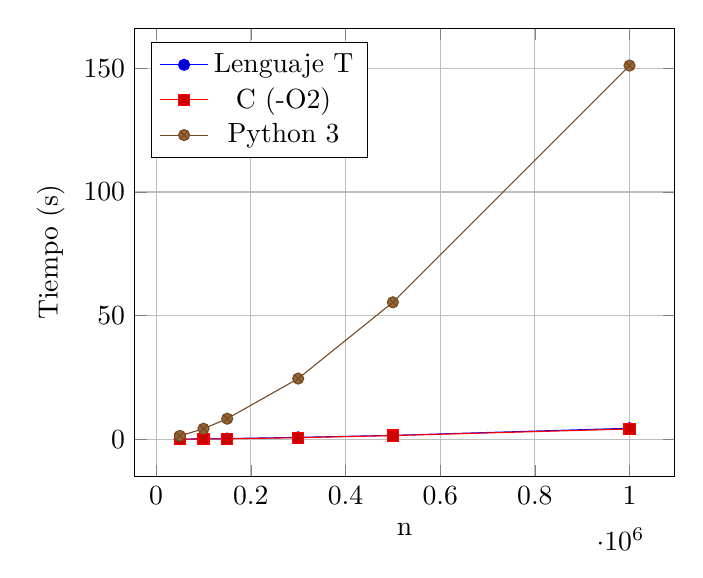
\begin{tikzpicture}
\begin{axis}[
    xlabel={n},
    ylabel={Tiempo (s)},
    legend pos=north west,
    grid=major
]
\addplot coordinates {
    (50000,0.046)
    (100000,0.156)
    (150000,0.279)
    (300000,0.774)
    (500000,1.579)
    (1000000,4.464)
};
\addlegendentry{Lenguaje T}

\addplot coordinates {
    (50000,0.059)
    (100000,0.126)
    (150000,0.218)
    (300000,0.636)
    (500000,1.509)
    (1000000,4.168)
};
\addlegendentry{C (-O2)}

\addplot coordinates {
    (50000,1.388)
    (100000,4.263)
    (150000,8.332)
    (300000,24.553)
    (500000,55.395)
    (1000000,151.118)
};
\addlegendentry{Python 3}
\end{axis}
\end{tikzpicture}
\caption{Gráfica comparativa del rendimiento en el cálculo de números primos}
\end{figure}


Los resultados obtenidos muestran que el código generado por el compilador desarrollado presenta un rendimiento muy cercano al del código C optimizado, con diferencias aproximadas de TODO. En contraste, tanto el programa en C como el generado por el compilador superan ampliamente a Python, siendo los ejecutables compilados alrededor de un TODO más rápidos que el interpretado.

Estos resultados se explican por el hecho de que tanto el lenguaje desarrollado como C generan código nativo que se ejecuta directamente sobre la arquitectura subyacente, sin la sobrecarga propia de los lenguajes interpretados. Asimismo, el uso de una representación intermedia eficiente y la delegación de las optimizaciones de bajo nivel en la infraestructura LLVM permiten obtener un rendimiento competitivo pese a tratarse de un compilador desarrollado en el contexto de un Trabajo de Fin de Grado.
